\chapter{Perancangan}
\label{chap:perancangan}

Pada bab ini akan dijelaskan mengenai perancangan aplikasi meliputi diagram kelas rinci beserta deskripsi dan fungsinya, dan perancangan antarmuka.

\section{Diagram Kelas Rinci} 
\label{sec:kelasdiagramrinci}
Diagram kelas rinci diperoleh dari hasil pengembangan diagram kelas analisis pada subbab \ref{sec:kelasdiagram}. Diagram kelas rinci dapat dilihat pada Gambar \ref{fig:4_kelas_diagram_rinci}. 

Deskripsi kelas beserta fungsi dari diagram kelas rinci tersebut adalah sebagai berikut:

\begin{enumerate}
	\item Application\\
	Kelas ini merupakan kelas yang sudah disediakan \play dan merupakan kelas Controller pada aplikasi KIRI. Atribut yang dimiliki kelas Application adalah:
	\begin{itemize}
		\item \textbf{DynamicForm dynamicForm:} objek DynamicForm yang berperan dalam mengambil query pada URL. 
		\item \textbf{WSClient ws:} objek WSClient yang berperan dalam memanggil layanan HTTP dari luar aplikasi KIRI.
		\item \textbf{Comparator<ArrayList<String>> comparator:} objek Comparator yang berperan dalam fungsi untuk membandingkan String dalam ArrayList.
		\item \textbf{CacheApi cache:} objek CacheApi yang berperan dalam mengambil data \textit{cache} yang telah dibuat oleh aplikasi KIRI.
		
	\end{itemize}
	\textit{Method-method} yang dimiliki kelas ini merupakan \textit{action method} dengan rincian sebagai berikut:
	\begin{itemize}
		\item \textbf{public Result index()}\\
		Berfungsi untuk mengarahkan pengguna ke halaman utama KIRI.\\
		\textbf{Kembalian:}  Halaman utama KIRI.
		
		\item \textbf{public Result handle()}\\
		Berfungsi untuk melakukan logikal data ketika pengguna mencari rute pada KIRI.\\
		\textbf{Kembalian:}  Halaman utama KIRI dengan hasil pencarian rute.
		
		\item \textbf{public String getFromMenjangan(String start,String finish,double mw,double wm,double pt)}\\
		Berfungsi untuk mendapatkan hasil dari menjangan.\\
		\textbf{Parameter:}
				\begin{itemize}
					\item \textbf{start} Lokasi awal pengguna.
					\item \textbf{finish} Lokasi akhir pengguna.
					\item \textbf{mw} Alternatif minimum walk.
					\item \textbf{wm} Alternatif walking multiplier.
					\item \textbf{pt} Alternatif penalty transfer.
				\end{itemize}.
				
		\textbf{Kembalian:}  Hasil dari layanan HTTP menjangan dengan query parameter.
		
		\item \textbf{public String getFromMenjangan(String start,String finish)}\\
		Berfungsi untuk mendapatkan hasil dari menjangan.\\
		\textbf{Parameter:}
				\begin{itemize}
					\item \textbf{start} Lokasi awal pengguna.
					\item \textbf{finish} Lokasi akhir pengguna.
				\end{itemize}.
				
		\textbf{Kembalian:}  Hasil dari layanan HTTP menjangan dengan query parameter.
		
		\item \textbf{public String getFromMenjangan(String start)}\\
		Berfungsi untuk mendapatkan hasil dari menjangan.\\
		\textbf{Parameter:}
				\begin{itemize}
					\item \textbf{start} Lokasi awal pengguna.
				\end{itemize}.
				
		\textbf{Kembalian:}  Hasil dari layanan HTTP menjangan dengan query parameter.
		
		\item \textbf{public String file\_get\_contents(String url)}\\
		Berfungsi untuk mendapatkan hasil dari URL tertentu.\\
		\textbf{Parameter:}
				\begin{itemize}
					\item \textbf{url} URL yang ingin didapatkan.
				\end{itemize}.
				
		\textbf{Kembalian:}  Hasil dari layanan HTTP dengan URL tertentu.
		
		\item \textbf{public String getPlacesAPI(String location,String radius,String querystring)}\\
		Berfungsi untuk mendapatkan hasil JSON dari maps.googleapis.com.\\
		\textbf{Parameter:}
				\begin{itemize}
					\item \textbf{location} Lokasi yang ingin dicari(garis lintang dan garis bujur).
					\item \textbf{radius} Radius dari lokasi yang ingin dicari.
					\item \textbf{querystring} Kata yang berkaitan dengan lokasi yang ingin dicari.
				\end{itemize}.
				
		\textbf{Kembalian:}  Hasil dari layanan HTTP menjangan dengan query parameter.
		
		\item \textbf{public String format\_traveltime(double time)}\\
		Berfungsi untuk melakukan format waktu.\\
		\textbf{Parameter:}
				\begin{itemize}
					\item \textbf{time} Waktu yang ingin diubah formatnya.
				\end{itemize}.
				
		\textbf{Kembalian:}  Hasil waktu yang sudah diformat.
		
		\item \textbf{public String retrieve\_data(String param)}\\
		Berfungsi untuk mendapatkan data dari query URL.\\
		\textbf{Parameter:}
				\begin{itemize}
					\item \textbf{param} Query yang ingin didapatkan.
				\end{itemize}.
				
		\textbf{Kembalian:}  Data pada query URL.
		
		\item \textbf{public boolean check\_apikey(String apikey)}\\
		Berfungsi untuk melakukan format waktu.\\
		\textbf{Parameter:}
				\begin{itemize}
					\item \textbf{apikey} Apikey yang ingin dicek.
				\end{itemize}.
				
		\textbf{Kembalian:}  Hasil pengecekan apikey layak dipakai atau tidak.
		
		\item \textbf{public String humanize\_point(String location)}\\
		Berfungsi untuk mendapatkan nama lokasi tempat dari titik koordinat lokasi.\\
		\textbf{Parameter:}
				\begin{itemize}
					\item \textbf{location} Titik koordinat lokasi.
				\end{itemize}.
				
		\textbf{Kembalian:}  Nama lokasi tempat.
		
		\item \textbf{public String format\_distanceltime(double time,String locale)}\\
		Berfungsi untuk melakukan format waktu berdasarkan lokalisasi.\\
		\textbf{Parameter:}
				\begin{itemize}
					\item \textbf{time} Waktu yang ingin diubah formatnya.
					\item \textbf{locale} Lokalisasi bahasa.
				\end{itemize}.
				
		\textbf{Kembalian:}  Hasil waktu yang sudah diformat sesuai lokalisasi.
	\end{itemize}
	\item Constants\\
	Kelas untuk mengisi variabel dengan konstanta dan berfungsi agar tidak menuliskan konstanta berulang kali dan membantu pengembangan aplikasi KIRI. Atribut yang dimiliki kelas Constants adalah:
	\begin{itemize}
		\item \textbf{Alternative[] alternatives:} Alternative dalam array.
		\item \textbf{Map<String,ProtoRegion> regioninfos:} Map yang terdiri dari kunci berupa String dan berisi objek ProtoRegion.
		\item \textbf{String cache\_geocoding:} Untuk mencari / menyimpan pada basisdata cache dengan type geocoding.
		\item \textbf{String cache\_searchplace:} Untuk mencari / menyimpan pada basisdata cache dengan type searchplace.
		\item \textbf{String places\_url:} URL googleapis untuk mencari nama lokasi tempat.
		\item \textbf{int search\_maxresult} Angka untuk perbandingan hasil pencarian.
		\item \textbf{String gmaps\_server\_key:} Kunci agar dapat akses googleapis.
		\item \textbf{String gmaps\_geocode\_url:} URL googleapis untuk mencari geokode lokasi tempat.
		\item \textbf{String angkotwebid\_url\_prefix:} Awalan URL untuk angkot.web.id.
		\item \textbf{String angkotwebid\_url\_suffix:} Akhiran URL untuk angkot.web.id.
		\item \textbf{int speed\_walk:} Kecepatan jalan kaki.
		\item \textbf{String proto\_attributions:} Untuk menampilkan JSON dengan kunci attributions. 
		\item \textbf{String proto\_errorcode:} Untuk mendapatkan query URL errorcode.
		\item \textbf{String proto\_location:} Untuk menyimpan pada HashMap dengan kunci location.
		\item \textbf{String proto\_message:} Untuk menampilkan JSON dengan kunci message.
		\item \textbf{String proto\_mode\_findroute:} Untuk mendapatkan query URL mode.
		\item \textbf{String proto\_mode\_reporterror:} Untuk mendapatkan query URL mode.
		\item \textbf{String proto\_mode\_search:} Untuk mendapatkan query URL mode.
		\item \textbf{String proto\_mode\_nearbytransports:} Untuk mendapatkan query URL mode.
		\item \textbf{String proto\_nearbytransports:} Untuk menampilkan JSON dengan kunci nearbytransports.
		\item \textbf{String proto\_placename:} Untuk menampilkan JSON dengan kunci placename.
		\item \textbf{String proto\_presentation\_desktop:} Untuk mengetahui apakah dibuka di desktop atau tidak.
		\item \textbf{String proto\_presentation\_mobile:} Untuk mengetahui apakah dibuka di mobile atau tidak.
		\item \textbf{String proto\_region:} Untuk mendapatkan query URL region.
		\item \textbf{String proto\_region\_bandung:} Region bandung dengan kode bdo.
		\item \textbf{String proto\_region\_jakarta:} Region bandung dengan kode jkt.
		\item \textbf{String proto\_region\_surabaya:} Region bandung dengan kode sby.
		\item \textbf{String proto\_region\_malang:} Region bandung dengan kode mlg.
		\item \textbf{String proto\_routestart:} Untuk mendapatkan query URL start.
		\item \textbf{String proto\_routingresult:} Untuk menampilkan JSON dengan kunci routingresult.
		\item \textbf{String proto\_routingresults:} Untuk menampilkan JSON dengan kunci routingresults.
		\item \textbf{String proto\_search\_querystring:} Untuk mendapatkan query URL querystring.
		\item \textbf{String proto\_search\_result:} Untuk menampilkan JSON dengan kunci searchresult.
		\item \textbf{String proto\_status:} Untuk menampilkan JSON dengan kunci status.
		\item \textbf{String proto\_status\_error:} Untuk menampilkan JSON dengan nilai error.
		\item \textbf{String proto\_status\_ok:} Untuk menampilkan JSON dengan nilai ok.
		\item \textbf{String proto\_steps:} Untuk menampilkan JSON dengan kunci steps.
		\item \textbf{String proto\_traveltime:} Untuk menampilkan JSON dengan kunci traveltime.
		\item \textbf{String protokd\_point\_finish:} Untuk pengecekan bila hasil dari menjangan ada kata finish.
		\item \textbf{String protokd\_point\_start:} Untuk pengecekan bila hasil dari menjangan ada kata start.
		\item \textbf{String protokd\_point\_finish:} Untuk pengecekan bila hasil dari menjangan ada kata finish.
		\item \textbf{String protokd\_transitmode\_walk:} Untuk pengecekan bila hasil dari menjangan ada kata walk.
	\end{itemize}
	
	
	\item Alternative\\
	Kelas yang merupakan turunan dari kelas yang sudah disediakan \play, yaitu Models. Kelas ini untuk merepresentasikan alternatif dalam pencarian rute pada URL \textit{http://newmenjangan.cloudapp.net:8000}. Kelas Alternative mempunyai atribut antara lain:
	\begin{itemize}
		\item \textbf{double mw:} Maximumwalk dari alternatif.
		\item \textbf{double wm:} Walkingmultiplier dari alternatif.
		\item \textbf{double pt:}  Penaltrytransfer dari alternatif.
	\end{itemize}
	
	\textit{Method-method} yang dimiliki kelas ini merupakan \textit{action method} dengan rincian sebagai berikut:
	\begin{itemize}
		\item \textbf{public double getPt()}\\
		Berfungsi untuk mendapatkan atribut pt.\\
		\textbf{Kembalian:}  Nilai pt.
		
		\item \textbf{public double getWm()}\\
		Berfungsi untuk mendapatkan atribut wm.\\
		\textbf{Kembalian:}  Nilai wm.
		
		\item \textbf{public double getMw()}\\
		Berfungsi untuk mendapatkan atribut mw.\\
		\textbf{Kembalian:}  Nilai mw.
	\end{itemize}
	
	\item ProtoRegion\\
	Kelas yang merupakan turunan dari kelas yang sudah disediakan \play, yaitu Models. Kelas ini untuk merepresentasikan kota dengan masing-masing mempunyai atribut sendiri. Kelas ProtoRegion mempunyai atribut antara lain:
	\begin{itemize}
		\item \textbf{double lat:} Titik lintang dari kota tertentu.
		\item \textbf{double lon:} Titik bujur dari kota tertentu.
		\item \textbf{int radius:}  Radius dari kota tertentu.
		\item \textbf{int zoom:}  Tingkat \textit{zoom} dari kota tertentu.
		\item \textbf{String searchPlace\_regex:}  \textit{Regex} dari kota tertentu guna dalam pencarian nama lokasi.
		\item \textbf{String name:}  Nama dari kota tertentu.
	\end{itemize}
	
	\textit{Method-method} yang dimiliki kelas ini merupakan \textit{action method} dengan rincian sebagai berikut:
	\begin{itemize}
		\item \textbf{public double getLat()}\\
		Berfungsi untuk mendapatkan atribut titik lintang.\\
		\textbf{Kembalian:}  Nilai titik lintang.
		
		\item \textbf{public double getLon()}\\
		Berfungsi untuk mendapatkan atribut titik bujur.\\
		\textbf{Kembalian:}  Nilai titik bujur.
		
		\item \textbf{public int getZoom()}\\
		Berfungsi untuk mendapatkan atribut tingkat \textit{zoom}.\\
		\textbf{Kembalian:}  Nilai \textit{zoom}.
		
		\item \textbf{public int getRadius()}\\
		Berfungsi untuk mendapatkan atribut radius.\\
		\textbf{Kembalian:}  Nilai radius.
		
		\item \textbf{public String getSearchPlace\_regex()}\\
		Berfungsi untuk mendapatkan atribut \textit{regex}.\\
		\textbf{Kembalian:}  Nilai \textit{regex}.
		
		\item \textbf{public String getName()}\\
		Berfungsi untuk mendapatkan atribut nama.\\
		\textbf{Kembalian:}  Nilai nama.
	\end{itemize}
	
	\item Utils\\
	Kelas yang merupakan kelas pembantu untuk fungsi-fungsi dalam aplikasi KIRI. Kelas Utils mempunyai \textit{Method-method} dengan rincian sebagai berikut:
	\begin{itemize}
	
		\item \textbf{public static void log\_statistic(String verifier,String type,String additional\_info)}\\
		Berfungsi untuk memasukkan data dalam basisdata statistic.\\
		\textbf{Parameter:}
				\begin{itemize}
					\item \textbf{verifier} Apikey yang mengisi data ke tabel.
					\item \textbf{type} Tipe statistic.
					\item \textbf{additional\_info} Keterangan statistik.
				\end{itemize}.
		\textbf{Kembalian:}  Tidak ada.
		
		\item \textbf{public static boolean domain\_matches(String url,String filter)}\\
		Berfungsi untuk pengecekan URL dengan filter sama atau tidak.\\
		\textbf{Parameter:}
				\begin{itemize}
					\item \textbf{url} Apikey yang mengisi data ke tabel.
					\item \textbf{filter} Filter untuk URL.
				\end{itemize}.
		\textbf{Kembalian:}  \texttt{true} jika URL sama dengan filter, \texttt{false} jika tidak sama.
	
		\item \textbf{public static boolean pregMatch(String regex, String content)}\\
		Berfungsi untuk pengecekan apakah dalam suatu kalimat mengandung kata tertentu.\\
		\textbf{Parameter:}
				\begin{itemize}
					\item \textbf{regex} Kata yang ingin dicari.
					\item \textbf{content} Kalimat yang ingin dicari.
				\end{itemize}.
		\textbf{Kembalian:}  \texttt{true} jika terdapat kata dalam kalimat, \texttt{false} jika tidak ada.
		
		\item \textbf{public static int indexPregMatch(String regex, String content)}\\
		Berfungsi untuk mengambil indeks kata tertentu dalam suatu kalimat jika ada.\\
		\textbf{Parameter:}
				\begin{itemize}
					\item \textbf{regex} Kata yang ingin dicari.
					\item \textbf{content} Kalimat yang ingin dicari.
				\end{itemize}.
		\textbf{Kembalian:}  Index kata tersebut dalam kalimat.
		
		\item \textbf{public static ObjectNode die\_nice(String message)}\\
		Berfungsi untuk mengembalikan JSON dengan status error dan message.\\
		\textbf{Parameter:}
				\begin{itemize}
					\item \textbf{message} Message yang ingin dituliskan.
				\end{itemize}.
		\textbf{Kembalian:}  JSON dengan status error dan message.
		
		\item \textbf{public static ObjectNode well\_done(String message)}\\
		Berfungsi untuk mengembalikan JSON dengan status ok dan message(jika ada).\\
		\textbf{Parameter:}
				\begin{itemize}
					\item \textbf{message} Message yang ingin dituliskan.
				\end{itemize}.
		\textbf{Kembalian:}  JSON dengan status ok dan message.
		
		\item \textbf{public static String get\_from\_cache(String type, String key)}\\
		Berfungsi untuk mendapatkan nilai cacheValue dari tabel cache dengan tipe dan key tertentu.\\
		\textbf{Parameter:}
				\begin{itemize}
					\item \textbf{type} Tipe cache.
					\item \textbf{key} Key dari cache.
				\end{itemize}.
		\textbf{Kembalian:}  Nilai dari cacheValue.
	
		\item \textbf{public static void put\_to\_cache(String type, String key)}\\
		Berfungsi untuk menyimpan nilai cacheValue ke tabel cache dengan tipe dan key tertentu.\\
		\textbf{Parameter:}
				\begin{itemize}
					\item \textbf{type} Tipe cache.
					\item \textbf{key} Key dari cache.
				\end{itemize}.
		\textbf{Kembalian:}  Tidak ada.
	
		\item \textbf{public static double deg2rad(double deg)}\\
		Berfungsi untuk mengubah angka dalam satuan derajat dengan satuan radian.\\
		\textbf{Parameter:}
				\begin{itemize}
					\item \textbf{deg} Angka dalam satuan derajat yang ingin diubah.
				\end{itemize}.
		\textbf{Kembalian:}  Angka dalam satuan radian.
	
		\item \textbf{public static void log\_error(String message)}\\
		Berfungsi untuk melakukan log dengan pesan tertentu.\\
		\textbf{Parameter:}
				\begin{itemize}
					\item \textbf{message} Pesan yang ingin dilog.
				\end{itemize}.
		\textbf{Kembalian:}  Tidak ada.
		
		\item \textbf{public static String validateLocale(String locale)}\\
		Berfungsi untuk melakukan validasi locale yang didapat dari cache.\\
		\textbf{Parameter:}
				\begin{itemize}
					\item \textbf{locale} Input locale.
				\end{itemize}.
		\textbf{Kembalian:}  Locale yang sudah divalidasi.
		
		\item \textbf{public static String validateRegion(String region)}\\
		Berfungsi untuk melakukan validasi region yang didapat dari cache.\\
		\textbf{Parameter:}
				\begin{itemize}
					\item \textbf{region} Input region.
				\end{itemize}.
		\textbf{Kembalian:}  Region yang sudah divalidasi.
		
	\end{itemize}
	
\end{enumerate}


\begin{figure}[ht]
	\centering
	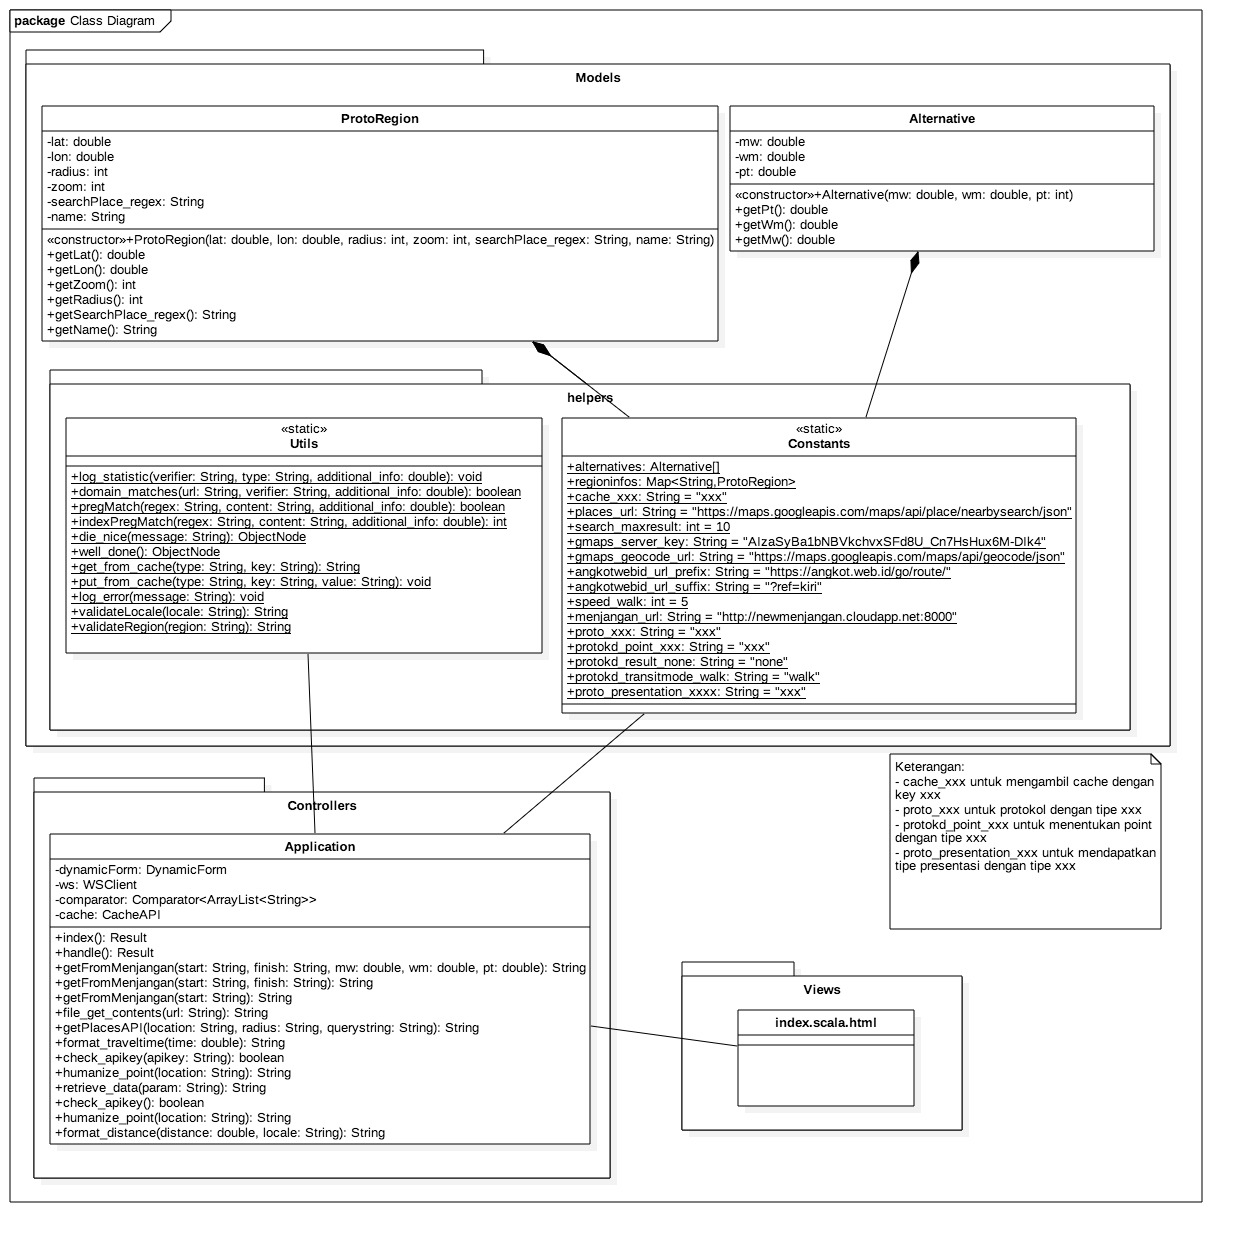
\includegraphics[scale=0.3]{Gambar/Class-Diagram-Rinci}
	\caption{Diagram Kelas Rinci} 
	\label{fig:4_kelas_diagram_rinci}
\end{figure}


\section{Perancangan Antarmuka}
\label{sec:perancangan_antarmuka}

Untuk memenuhi kebutuhan interaksi antara pengguna dengan sistem, maka dirancanglah sebuah antarmuka dari KIRI. Antarmuka mengikuti aplikasi KIRI yang lama. Rancangan antarmuka terdiri dari:

\begin{figure}[H]
	\centering
	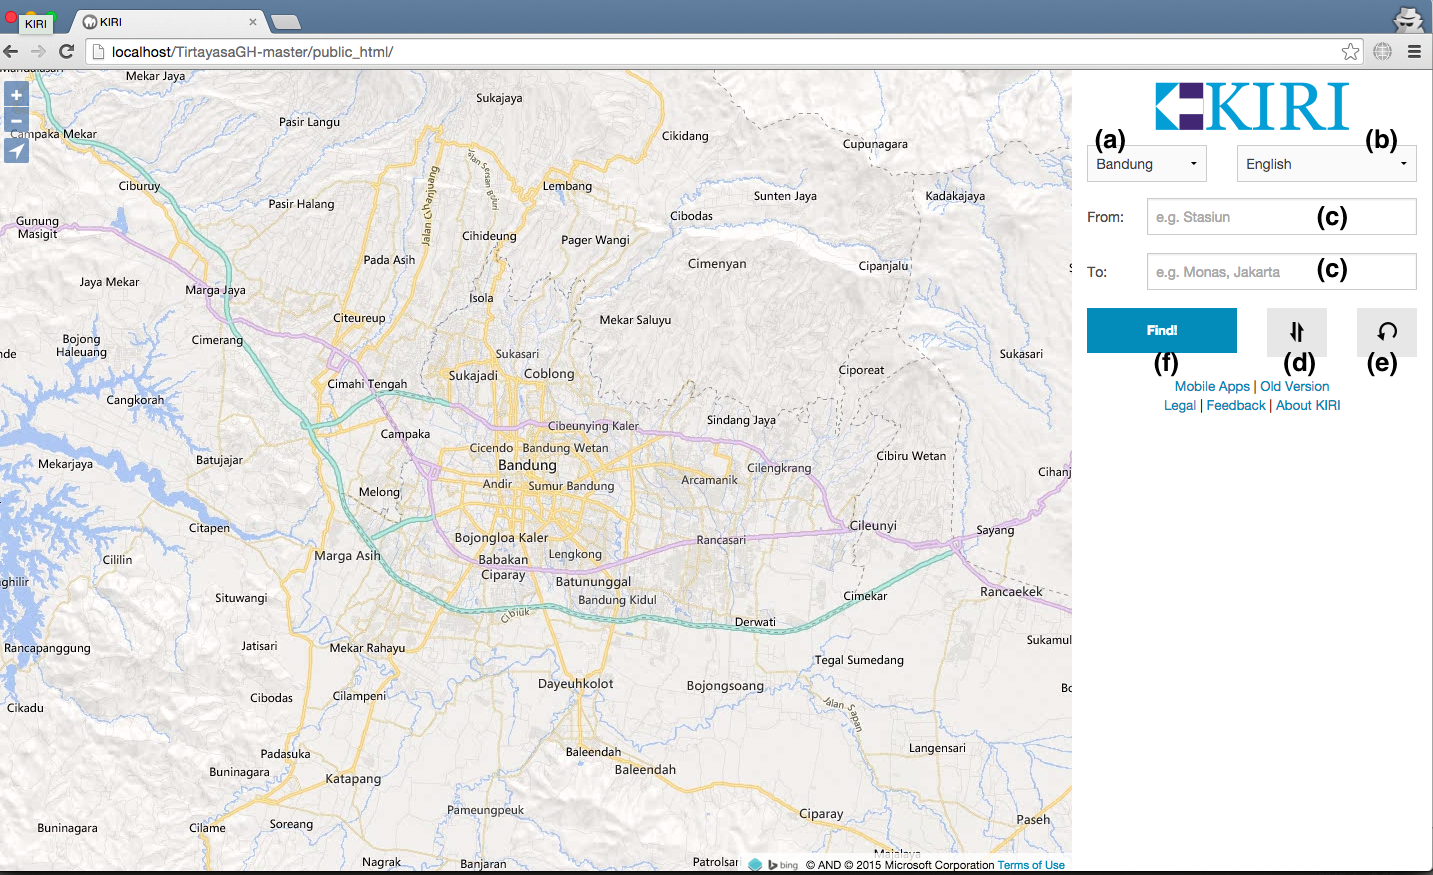
\includegraphics[scale=0.3]{Gambar/KIRI-main}
	\caption{Halaman Utama KIRI} 
	\label{fig:4_KIRI_main}
\end{figure}

Pada halaman utama KIRI (dapat dilihat pada gambar \ref{fig:4_KIRI_main}), terdapat beberapa bagian yaitu:
    \begin{enumerate}
    		\item \textbf{Peta}
    		\item \textbf{Form Samping} yang terdiri dari beberapa bagian, yaitu:
    		\begin{enumerate}
    			\item Dropdown Menu Kota
    			\item Dropdown Menu Bahasa
    			\item Textfield
    			\item Tombol Swap
    			\item Tombol Reset
    			\item Tombol Find
    		\end{enumerate}
    \end{enumerate}

\begin{figure}[H]
	\centering
	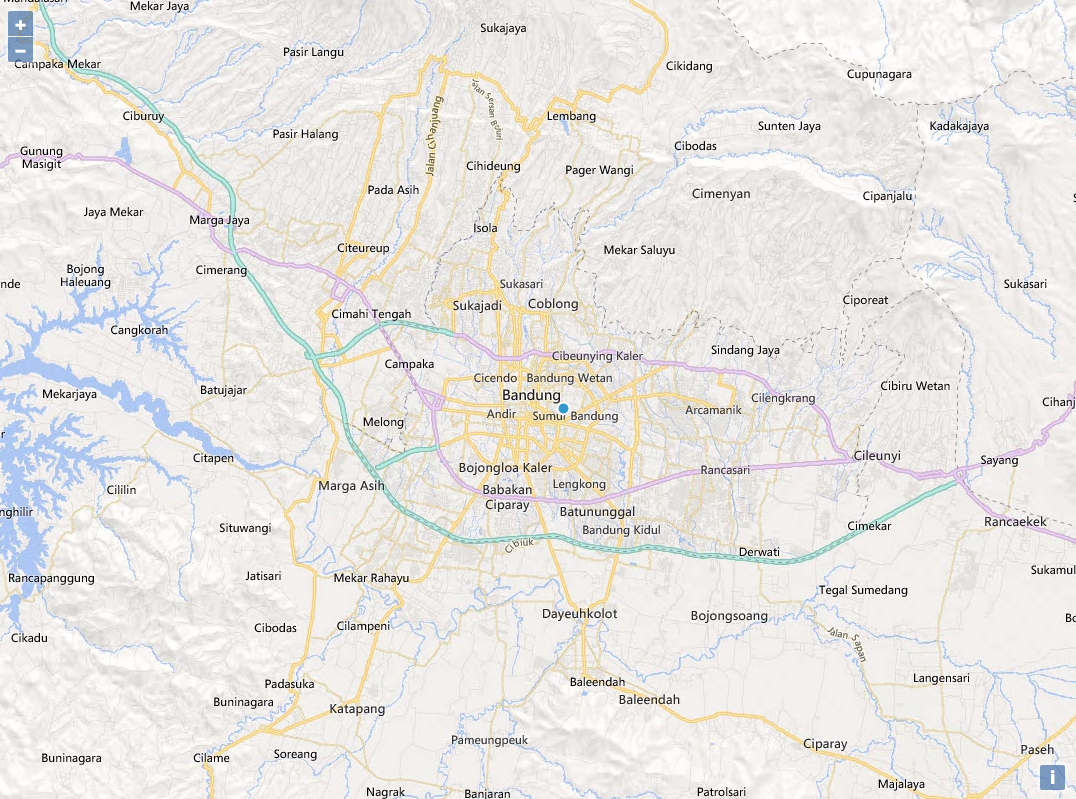
\includegraphics[scale=0.4]{Gambar/KIRI-peta}
	\caption{Peta pada KIRI} 
	\label{fig:4_KIRI_peta}
\end{figure}

\subsection{Peta}
Peta berfungsi untuk memudahkan pengguna dalam memilih lokasi awal dan lokasi akhir serta memberikan gambaran rute yang telah dicari oleh KIRI. KIRI menggunakan OpenLayers yang berbasis JavaScript untuk memuat peta pada halaman \textit{web}. 

\subsection{Form Samping}
Form yang terdapat pada halaman utama KIRI (Gambar \ref{fig:4_KIRI_form}) terdiri dari:
\begin{figure}[H]
	\centering
	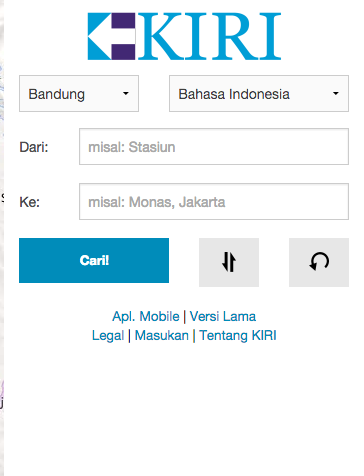
\includegraphics[scale=0.5]{Gambar/KIRI-form}
	\caption{Form pada KIRI} 
	\label{fig:4_KIRI_form}
\end{figure}

\subsubsection{Dropdown Menu Kota}
\textit{Dropdown} yang berfungsi untuk memilih kota yang akan ditampilkan pada peta dan memperbarui peta (Gambar \ref{fig:4_KIRI_drop_kota}).

\begin{figure}[H]
	\centering
	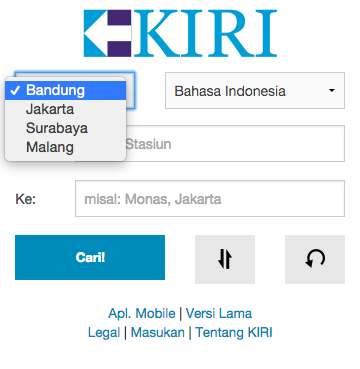
\includegraphics[scale=0.5]{Gambar/KIRI-drop-kota}
	\caption{Dropdown Menu Kota pada KIRI} 
	\label{fig:4_KIRI_drop_kota}
\end{figure}

\subsubsection{Dropdown Menu Bahasa}
\textit{Dropdown} yang berfungsi untuk memilih bahasa yang akan digunakan pada aplikasi KIRI (Gambar \ref{fig:4_KIRI_drop_bahasa}).

\begin{figure}[H]
	\centering
	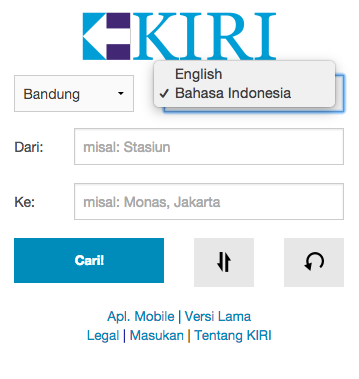
\includegraphics[scale=0.5]{Gambar/KIRI-drop-bahasa}
	\caption{Dropdown Menu Bahasa pada KIRI} 
	\label{fig:4_KIRI_drop_bahasa}
\end{figure}


\subsubsection{Textfield}
\textit{Textfield} pada KIRI agar pengguna dapat memasukkan \textit{input} sendiri. Textfield pada KIRI dapat menerima dua masukan pengguna, yaitu:

\begin{enumerate}
	\item \textbf{Textfield dengan Masukan Nama Tempat}, pengguna dapat memasukkan nama tempat asal dan tujuan (Gambar \ref{fig:4_KIRI_textfield_nama})
	
	\begin{figure}[H]
		\centering
		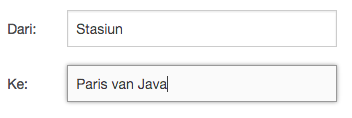
\includegraphics[scale=0.5]{Gambar/KIRI-textfield-nama}
		\caption{Input User(Nama Tempat)} 
		\label{fig:4_KIRI_textfield_nama}
	\end{figure}
	
	\item \textbf{Textfield dengan Masukan Klik Peta}, pengguna memasukkan koordinat tempat asal dan tujuan dengan klik pada peta. Dengan melakukan klik pada peta, textfield tempat asal dan tujuan akan akan secara otomatis terisi oleh koordinat masing-masing tempat (Gambar \ref{fig:4_KIRI_textfield_koord}).
	
	\begin{figure}[H]
		\centering
		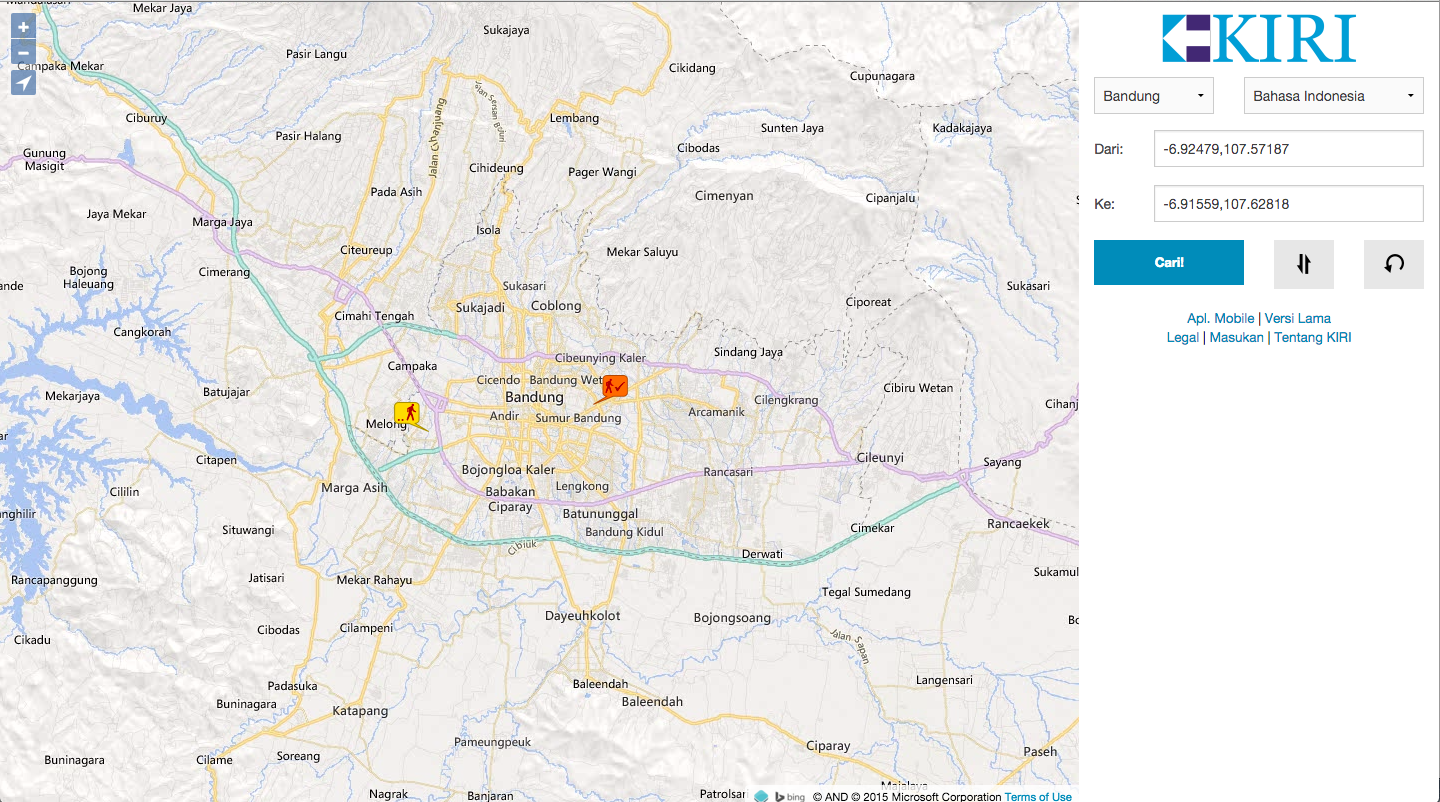
\includegraphics[scale=0.3]{Gambar/KIRI-textfield-koord}
		\caption{Input User(Klik pada peta)} 
		\label{fig:4_KIRI_textfield_koord}
	\end{figure}
	

\end{enumerate}

\subsubsection{Tombol Swap}
Pengguna dapat menukar isi dari \textit{textfield} tempat asal dan tujuan. 

\subsubsection{Tombol Reset}
Pengguna dapat melakukan pemilihan tempat dari awal dan mengulang tampilan peta. 

\subsubsection{Tombol Find}
Pengguna dapat mencari rute untuk sampai ke tujuan (Gambar \ref{fig:4_KIRI_find}). Pengguna dapat memilih rute alternatif yang sudah disediakan KIRI jika ada (Gambar \ref{fig:4_KIRI_find_alternate}).

\begin{figure}[H]
	\centering
	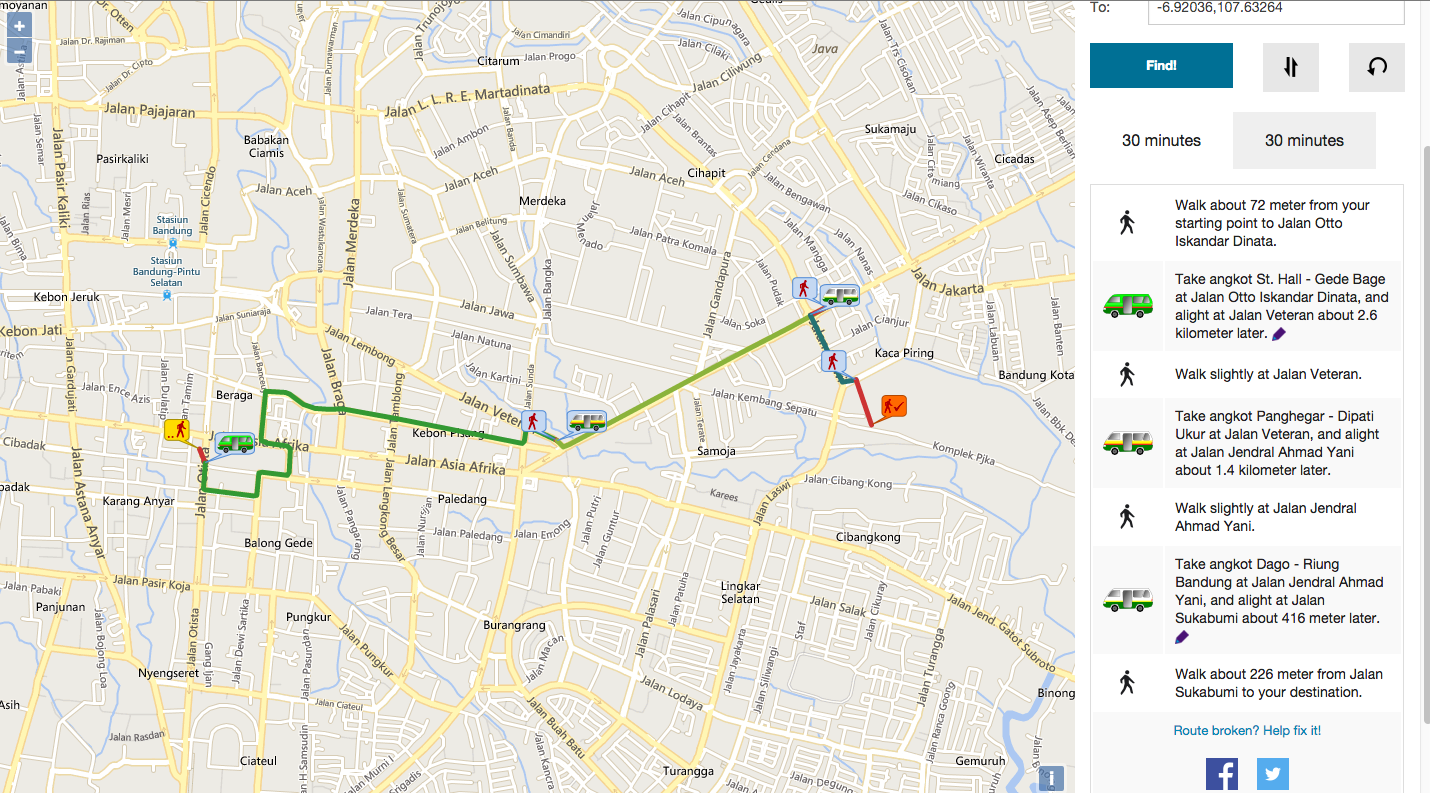
\includegraphics[scale=0.3]{Gambar/KIRI-find}
	\caption{Contoh Pencarian Rute pada KIRI} 
	\label{fig:4_KIRI_find}
\end{figure}

\begin{figure}[H]
	\centering
	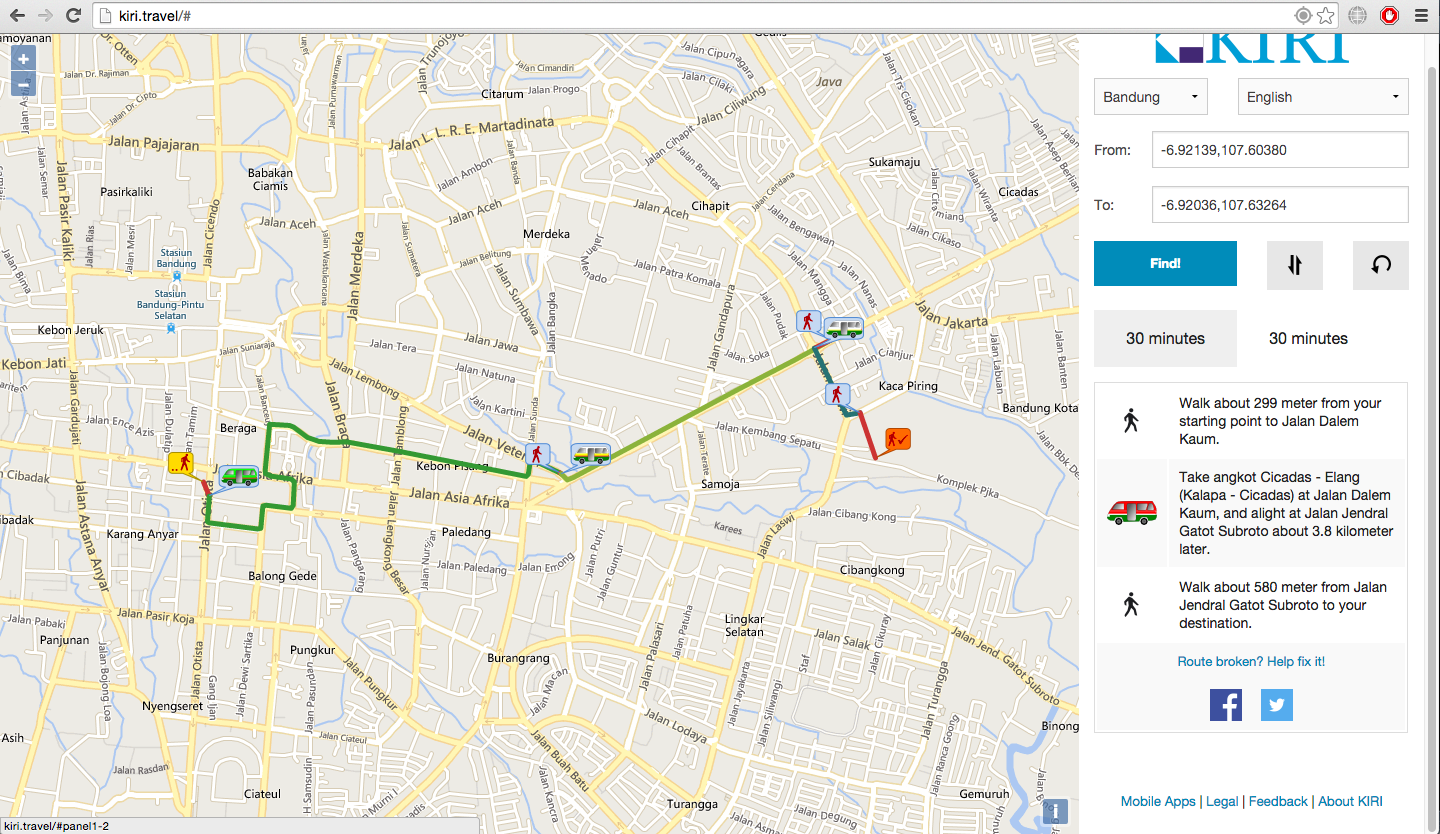
\includegraphics[scale=0.3]{Gambar/KIRI-find-alternate}
	\caption{Contoh Rute Alternatif pada KIRI} 
	\label{fig:4_KIRI_find_alternate}
\end{figure}
